\begin{appendices}
\chapter{\SB{} v1 Design Evaluation}
\label{app:evalutation}

Once \SB{} v1 was built and evaluated, the system performed mostly as designed.
Since this was an initial venture into building an untethered tensegrity robot, there were several design choices that ultimately impacted the system's performance negatively.
In the following sections, I will try to summarize and evaluate how the mechanical, electrical, and communication systemnjous performed.
I will then try to make suggestions to improve upon these systems.

\section{Mechanical Evaluation}

In this section, an evaluation of the \SB{} will be taken based on the three main subsystems outlined above.

\subsection{Cable Routing}
Upon testing and using \SB{}, the limitations on the mechanical design became the largest hindrance to achieving consistent performance.
A large majority of the mechanical limitations stemmed from the bowden cable routing, management, and material choices.
The design of the MTR was focused around using a bowden system to route cables around components and features within the housing.
This allowed for the cable routing to be secondary to the placement of components within the MTR, making the overall design easier, but increasing the number of bends in the bowden cable housing.
As explained in section \ref{routing}, the internal cable material used was braided steel cable.
The steel cable allowed for easy assembly and good wear resistance, however it has a minimum bend radius to keep the cable from plastically deforming.
Our initial design took into account this limitation with a correctly sized roller guide (see figure \ref{fig:roller_guide}), though in practice the combination of the induced tension and the wrong type of groove in the roller guide leads to a slight plastic deformation of the steel cable in the form of kinks.
Extra friction is then imparted into the bowden system as theses kinks try to slide inside the bowden housing.
Friction between the cable and housing element was a known factor, however the amount of friction it induced is much larger than expected.
Figure \ref{fig:cable_friction} shows a qualitative example of hysteresis in cable length due to the effect friction has on the system.

% \begin{figure}[thpb]
%       \centering
%       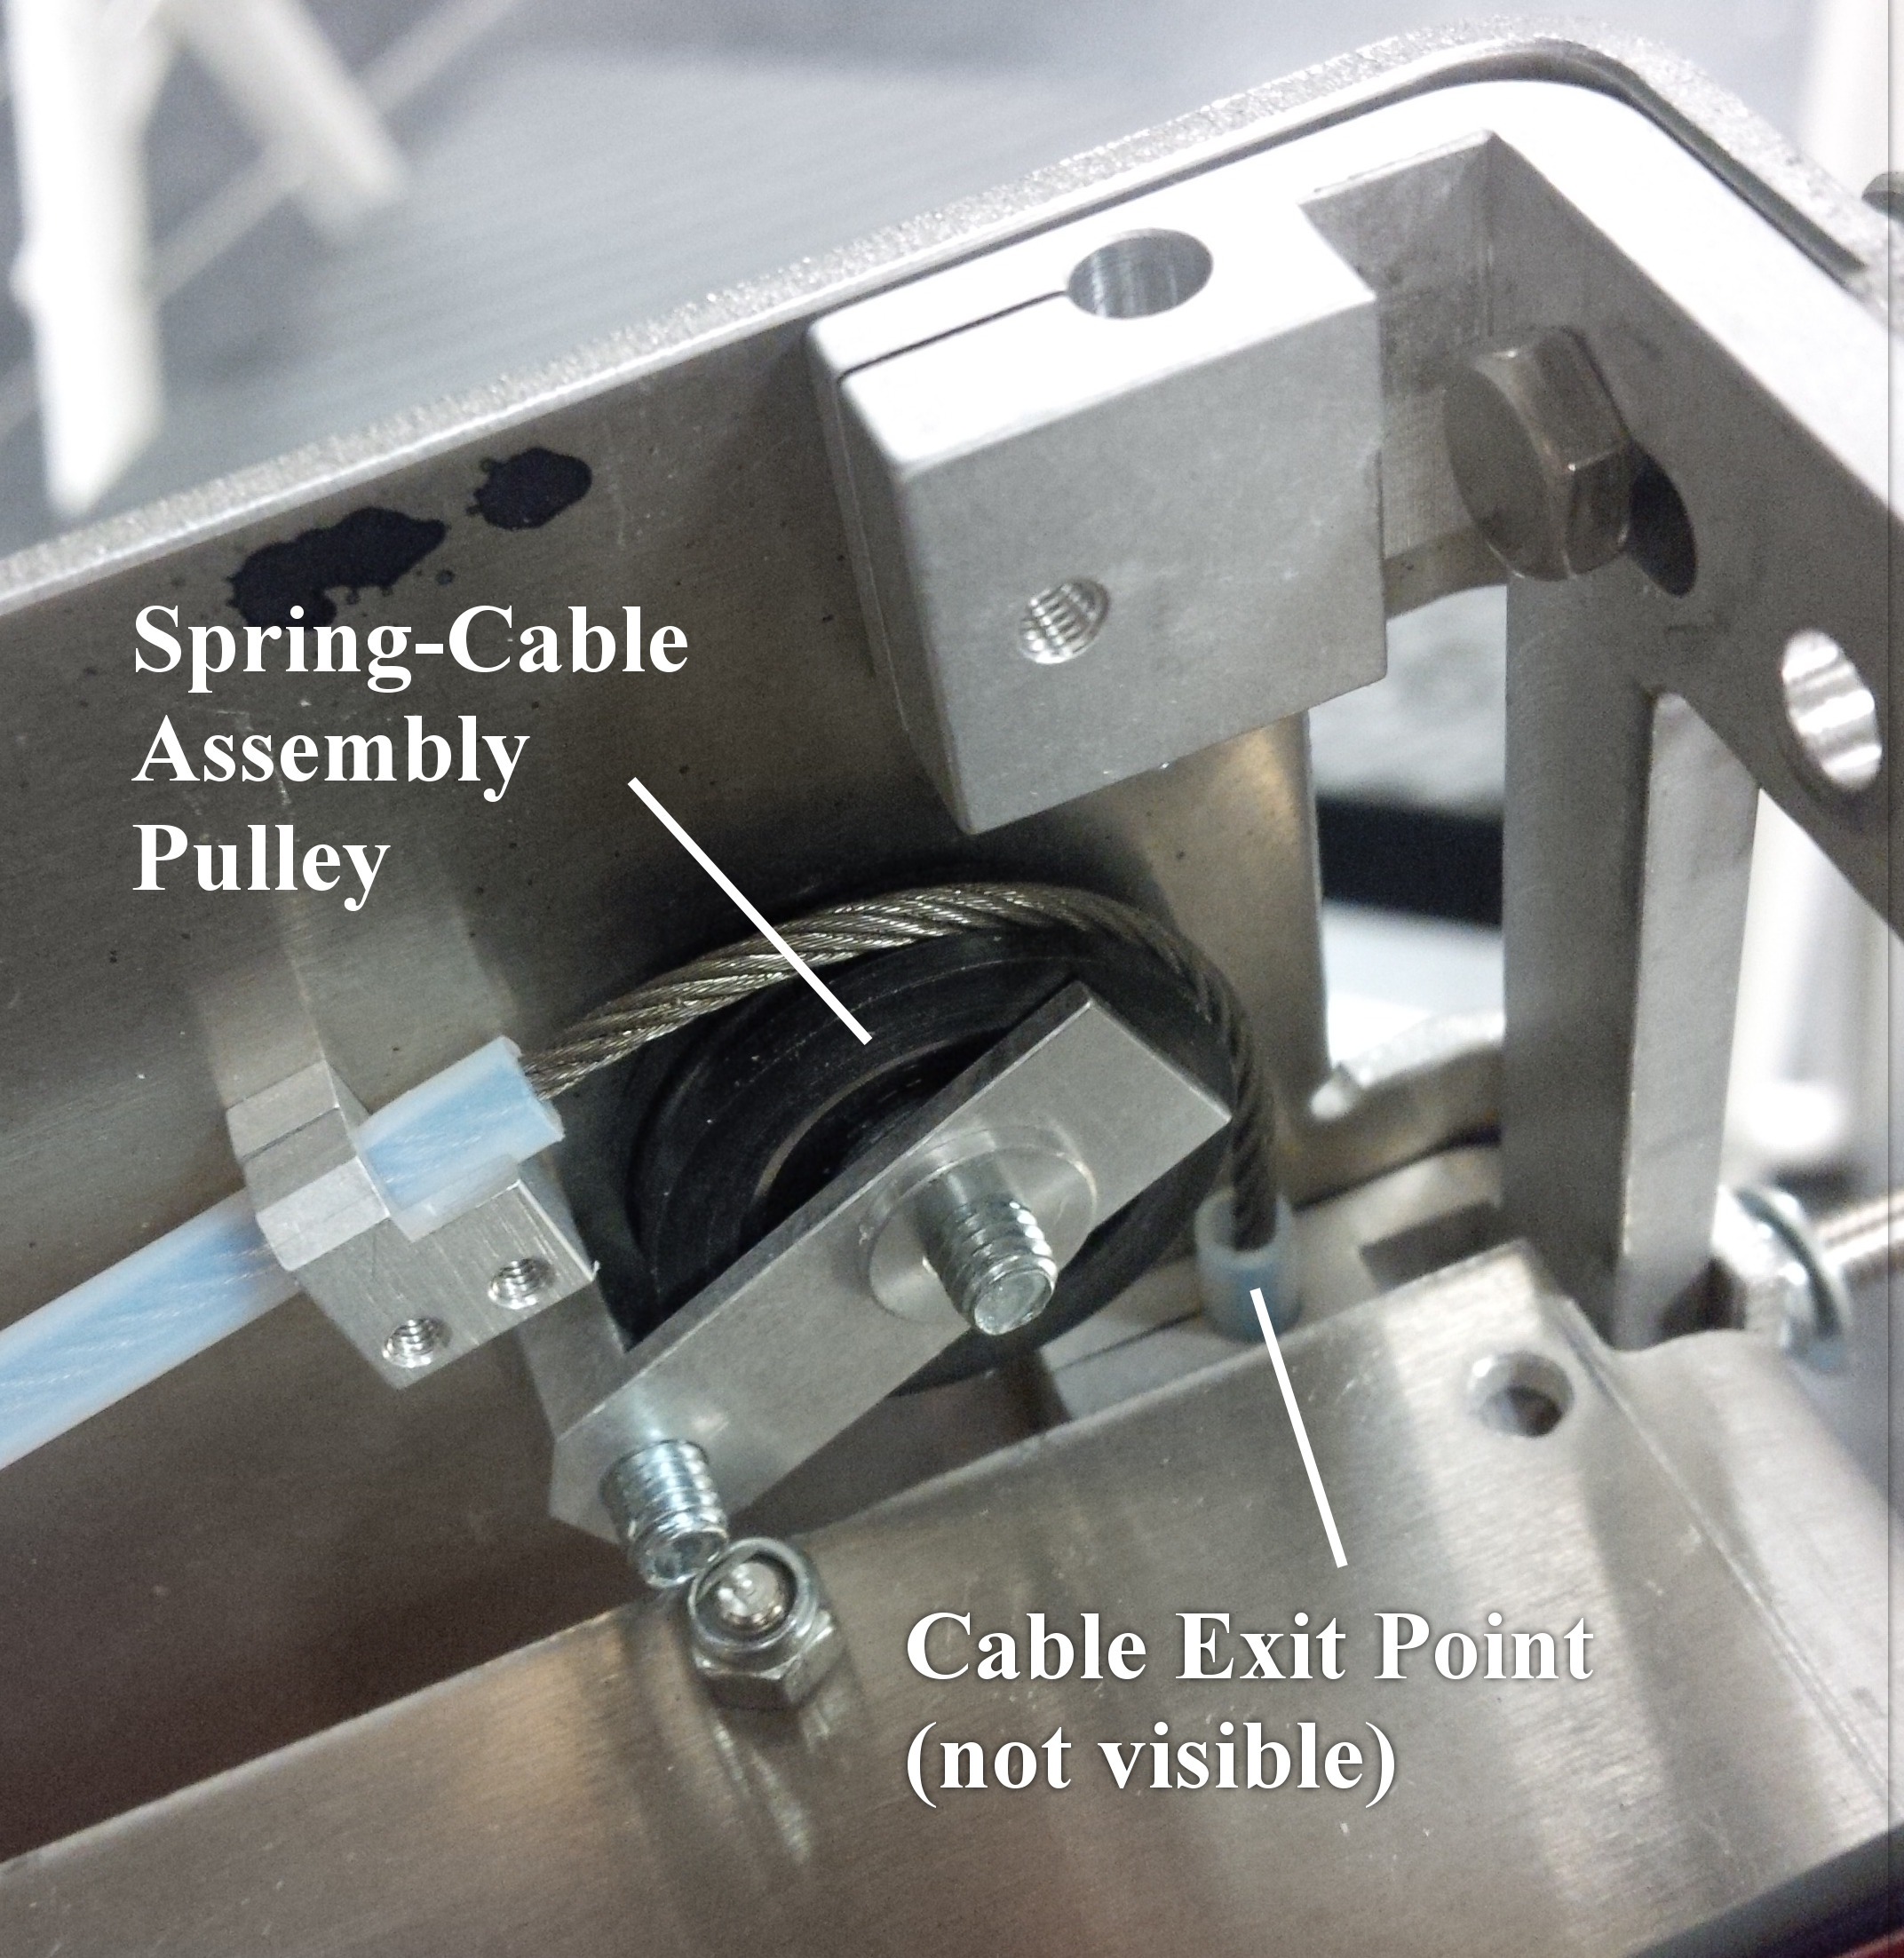
\includegraphics[width=0.6\columnwidth]{tex/img/cable_pulley_bearing_labelled_fixedfonts}
%       \caption{\textcolor{red}{Temp. figure. Explain how the pictures show hysteresis due to cable friction.}}
%       \label{fig:cable_friction}
% \end{figure}

\begin{figure}[htp] % not h only
\centering
\begin{subfigure}{.5\textwidth}
\centering
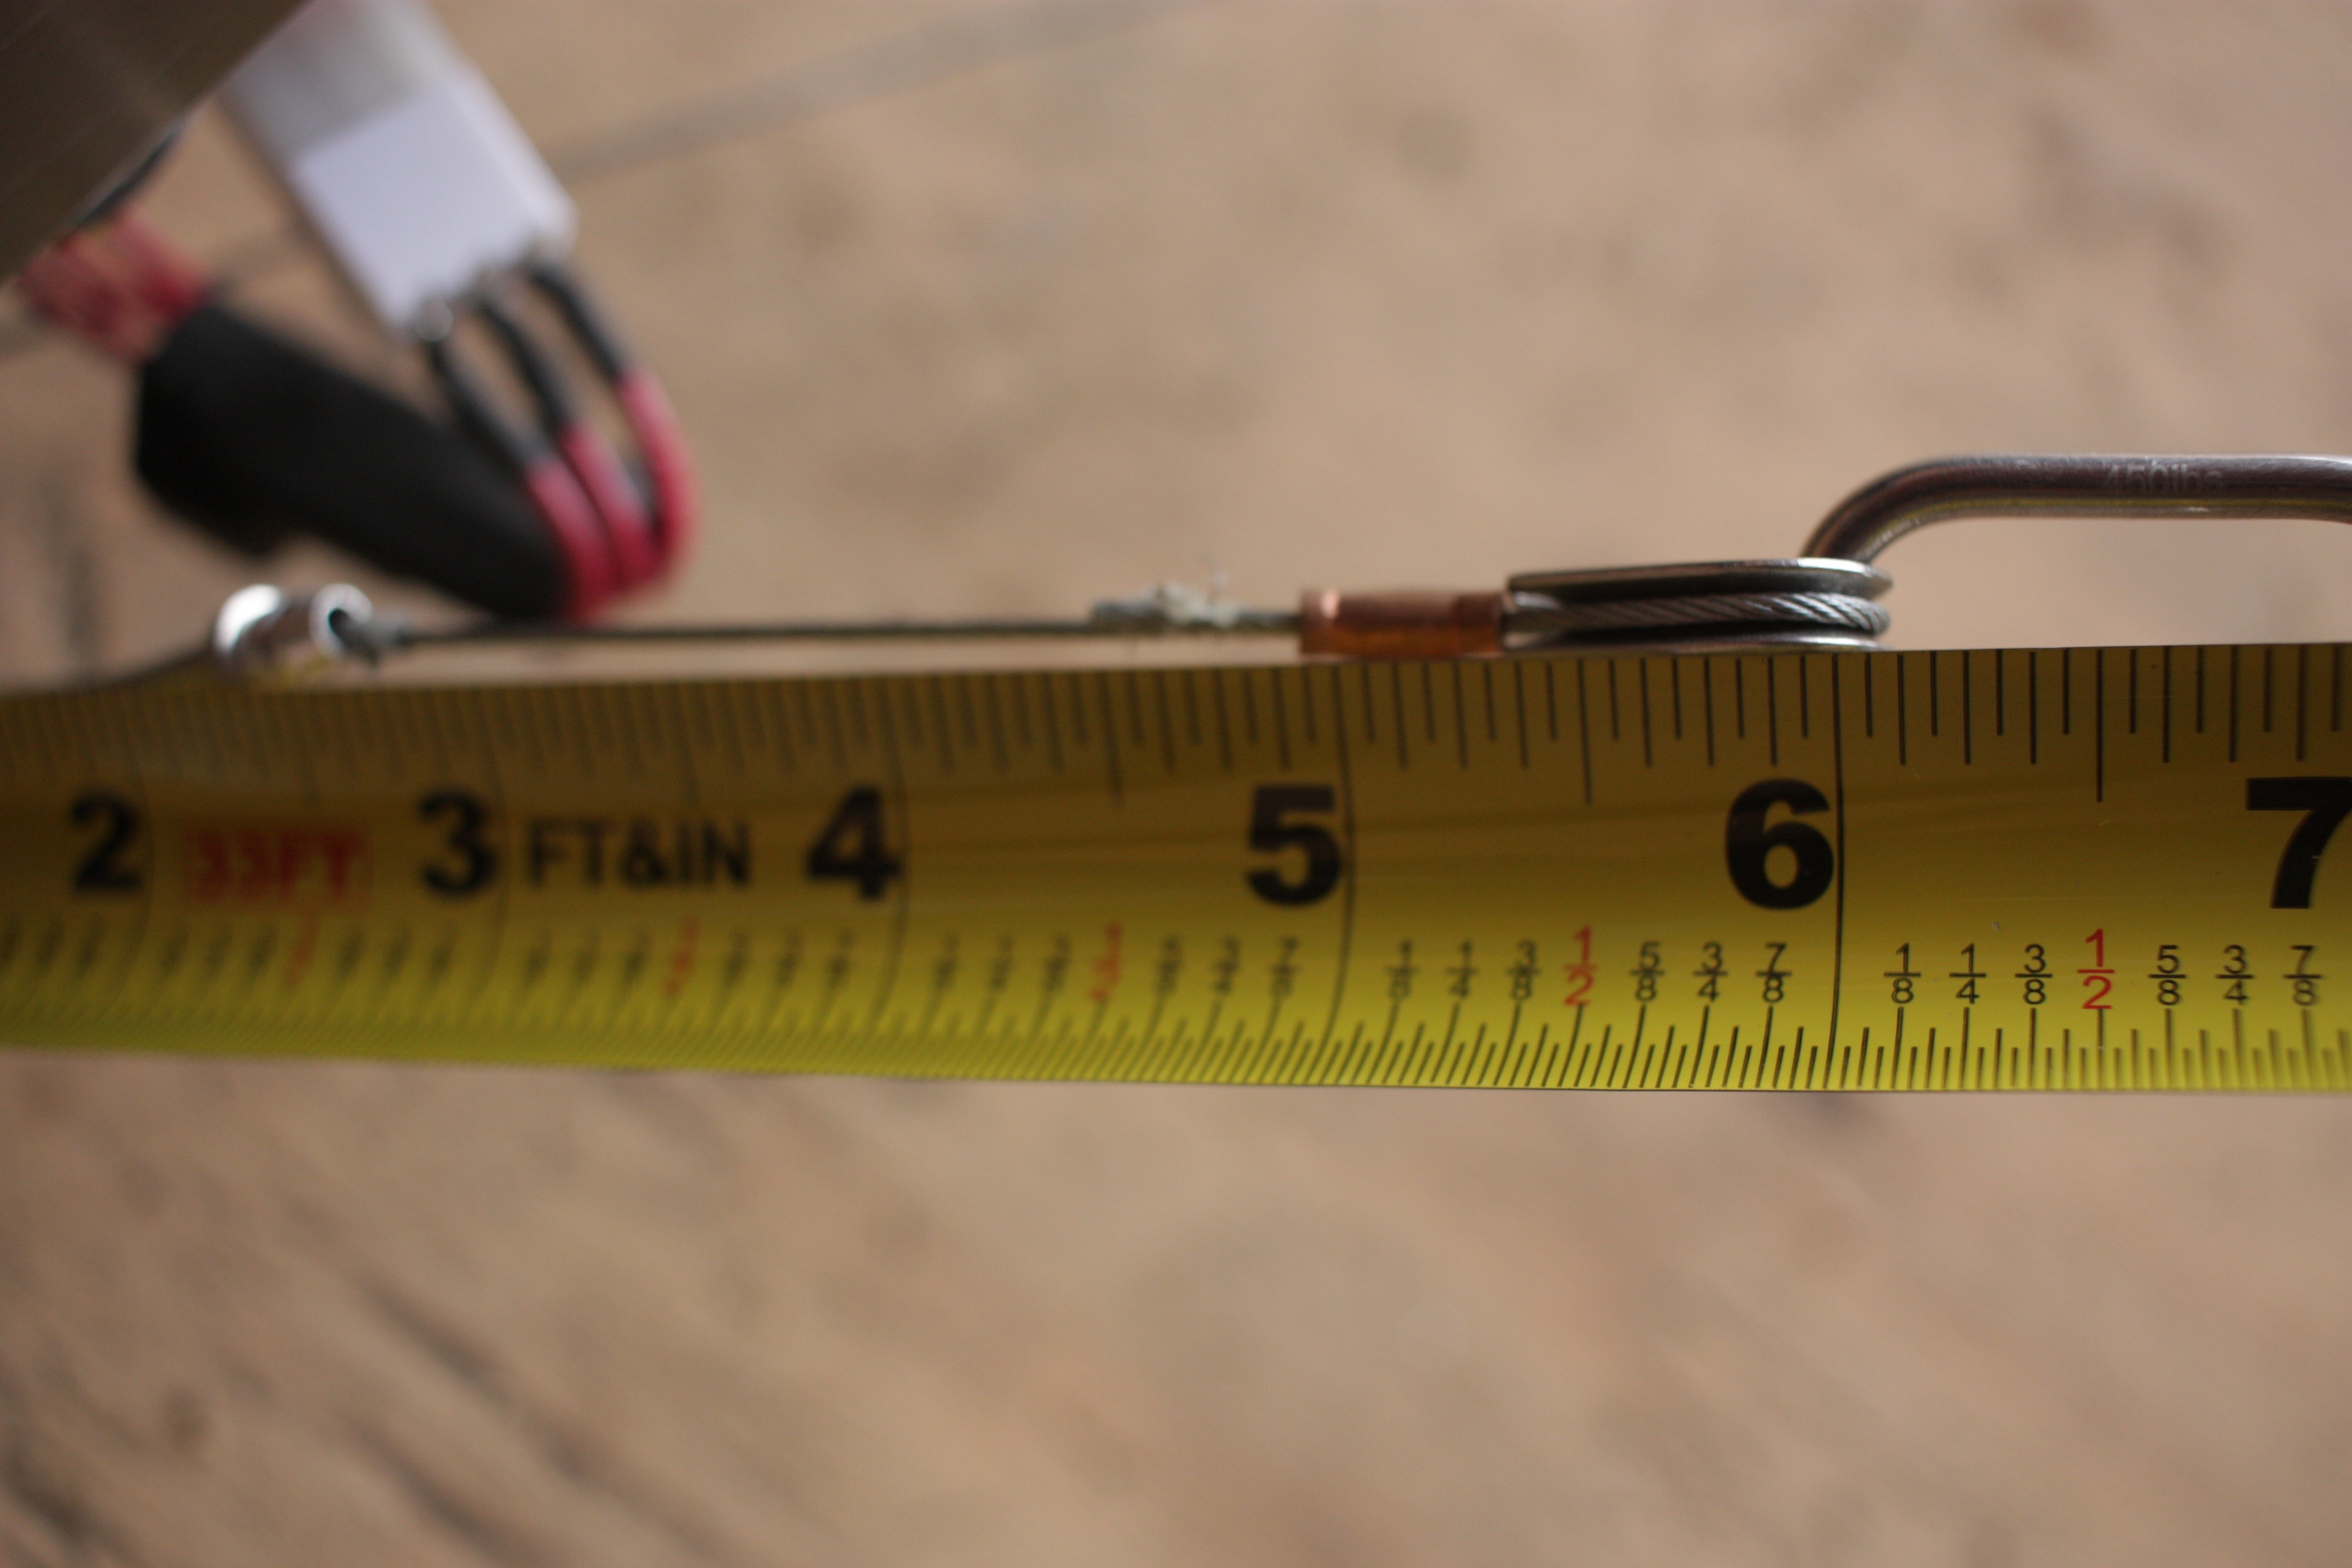
\includegraphics[width=0.9\linewidth]{tex/img/ruler_6}%
\label{fig:ruler_6}%
\end{subfigure}%
\begin{subfigure}{.5\textwidth}
\centering
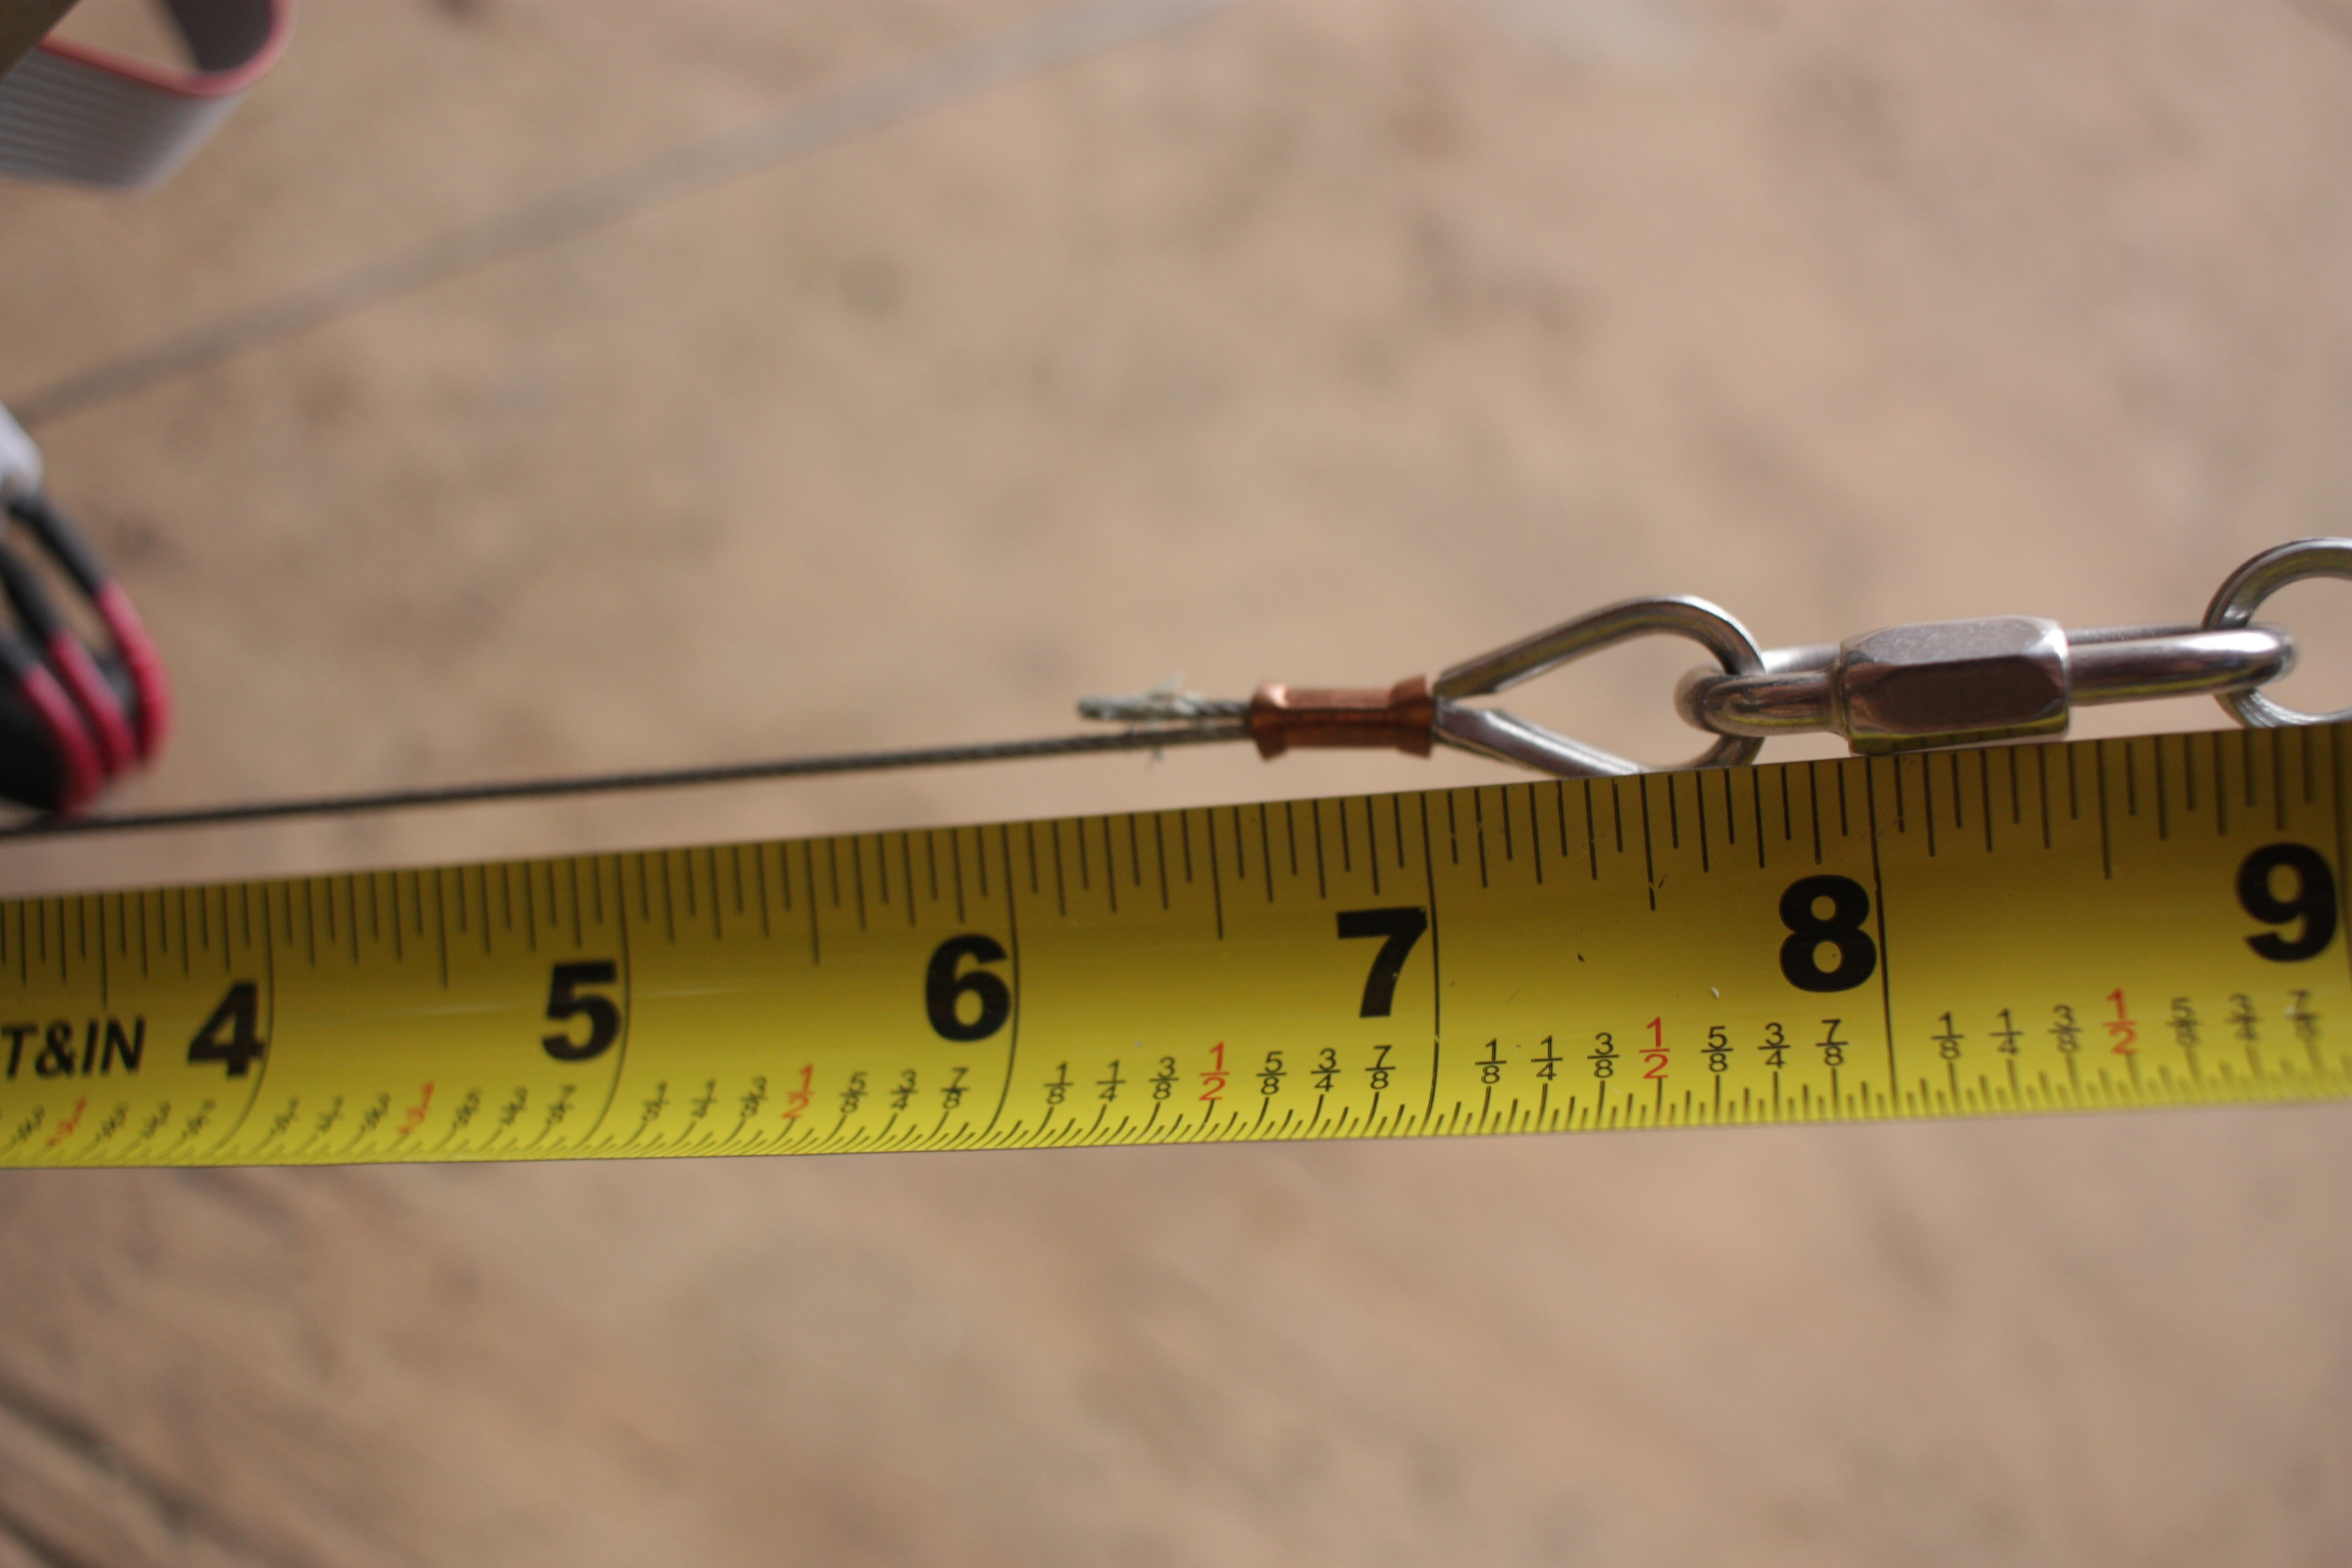
\includegraphics[width=0.9\linewidth]{tex/img/ruler_8}%
\label{fig:ruler_8}%
\end{subfigure}%

\begin{subfigure}{.5\textwidth}
\centering
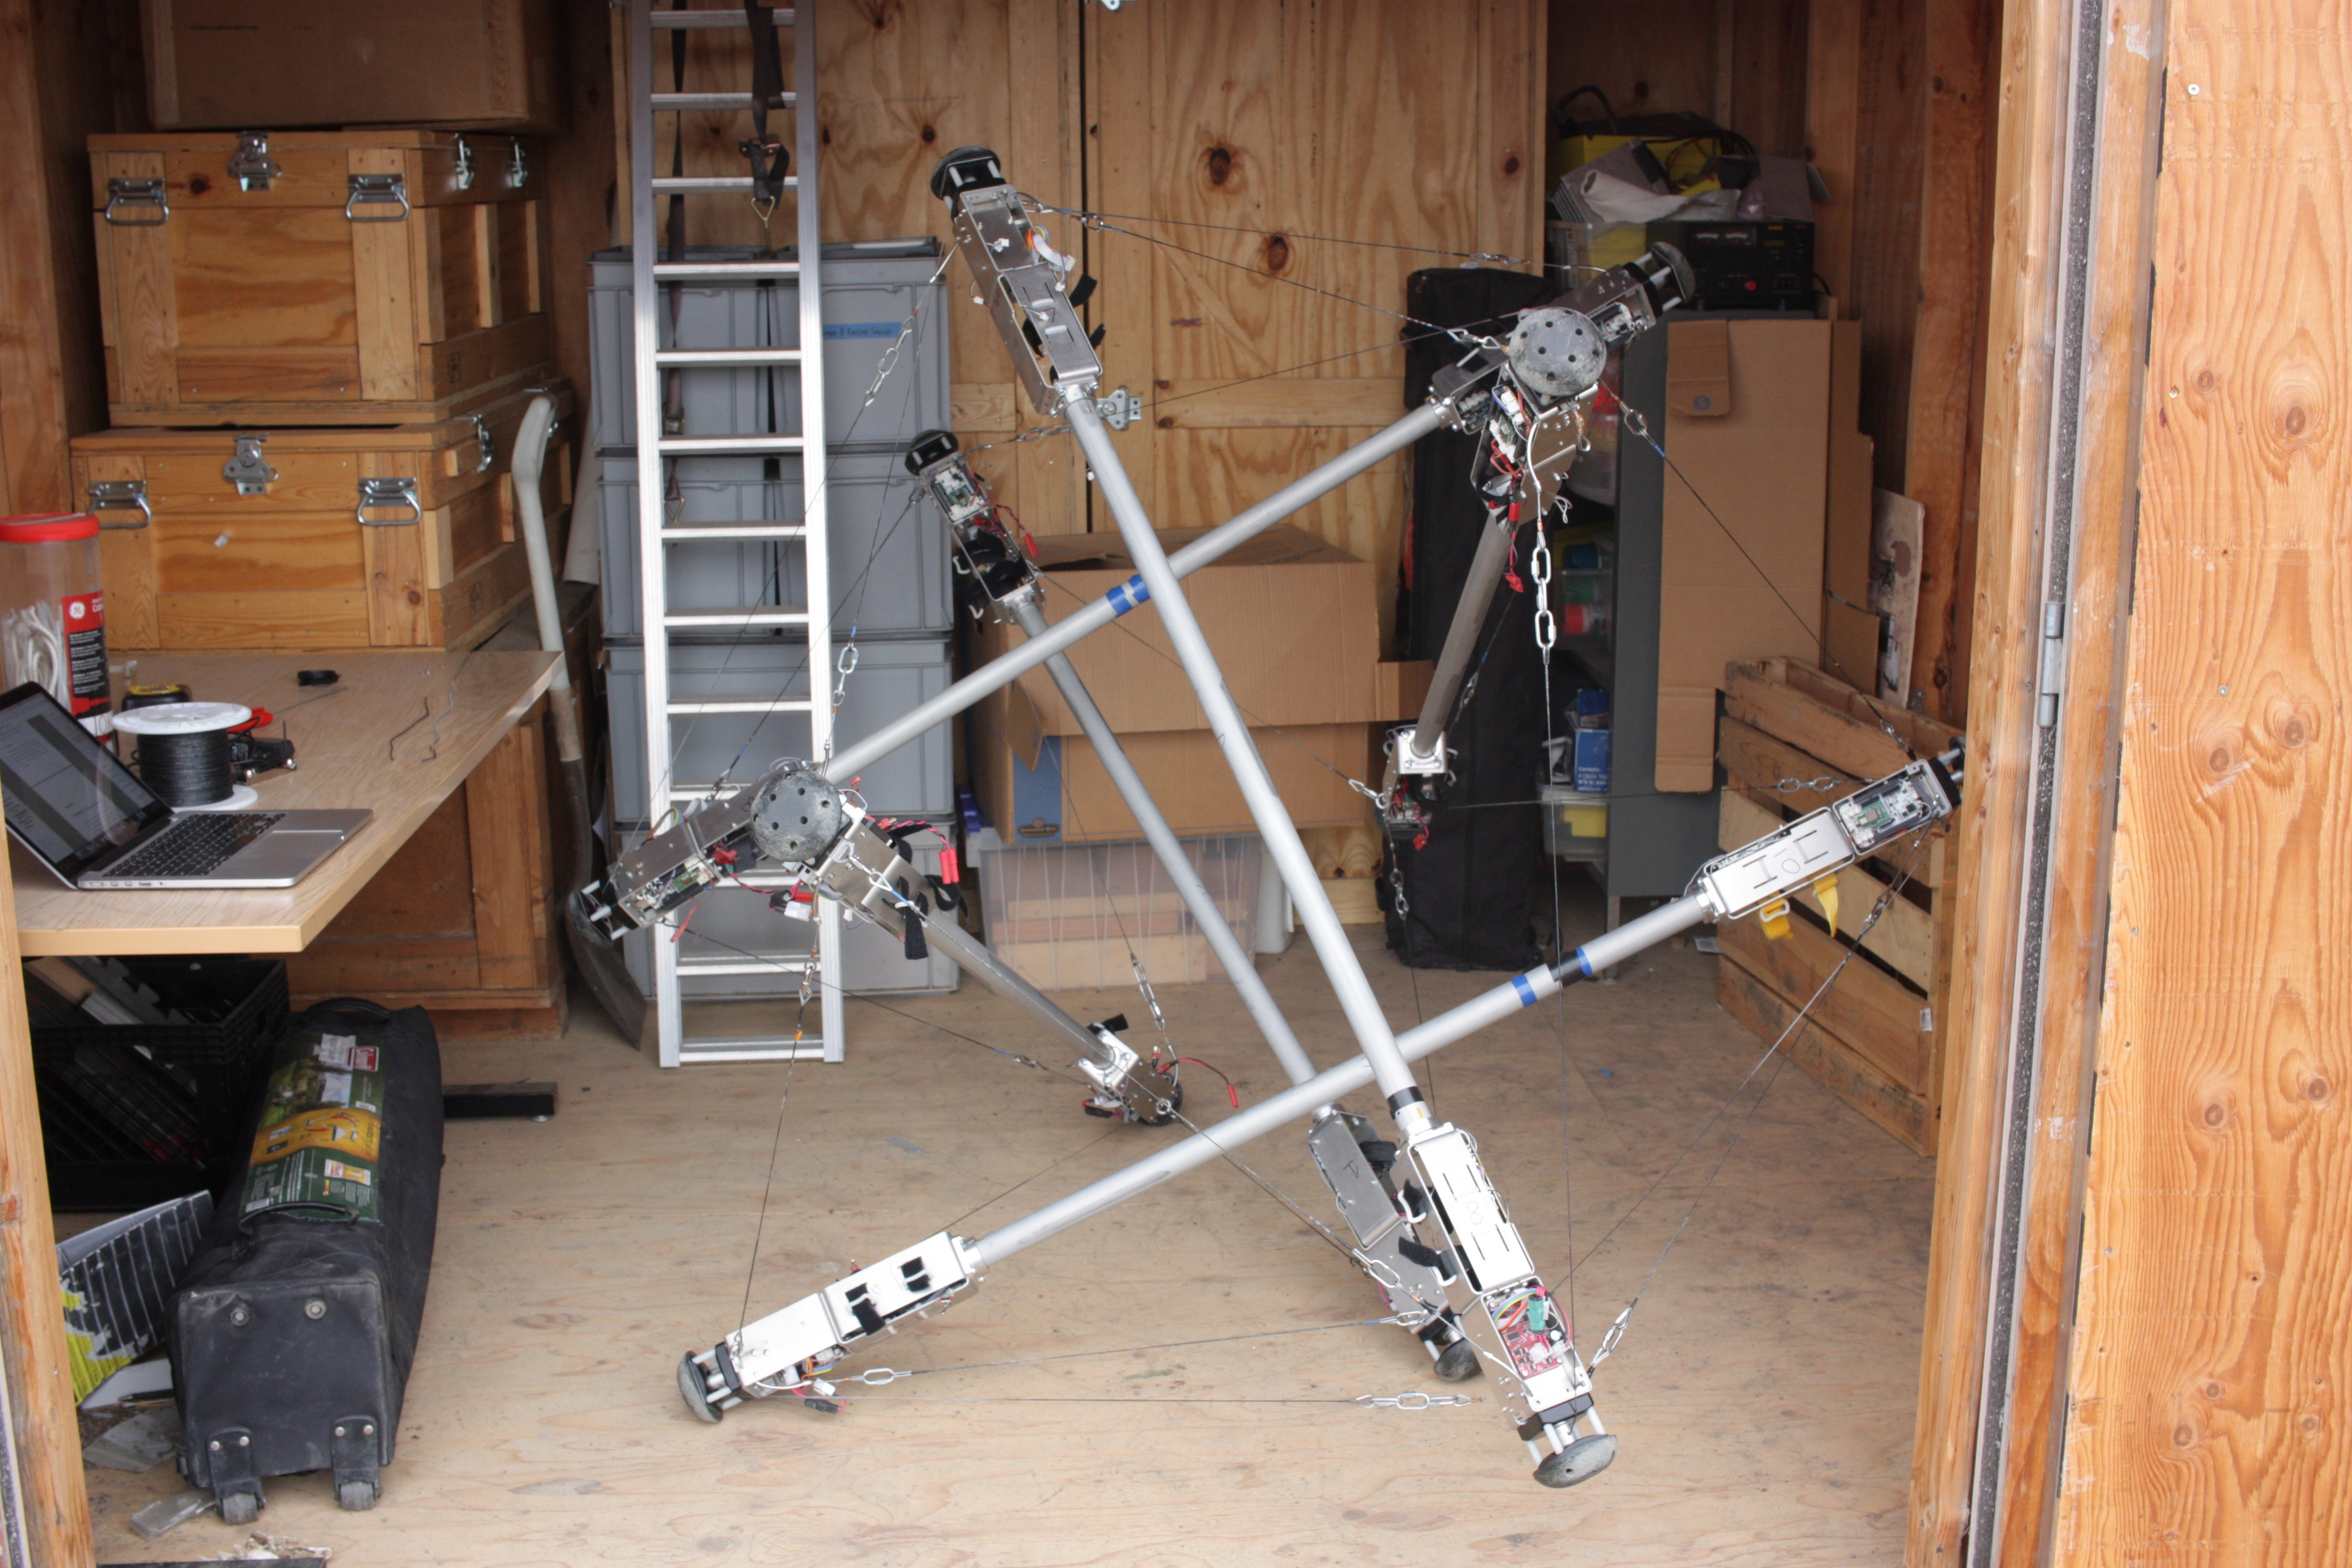
\includegraphics[width=0.9\linewidth]{tex/img/full_sb_up}%
\label{fig:sb_up}%
\caption{}
\end{subfigure}%
\begin{subfigure}{.5\textwidth}
\centering
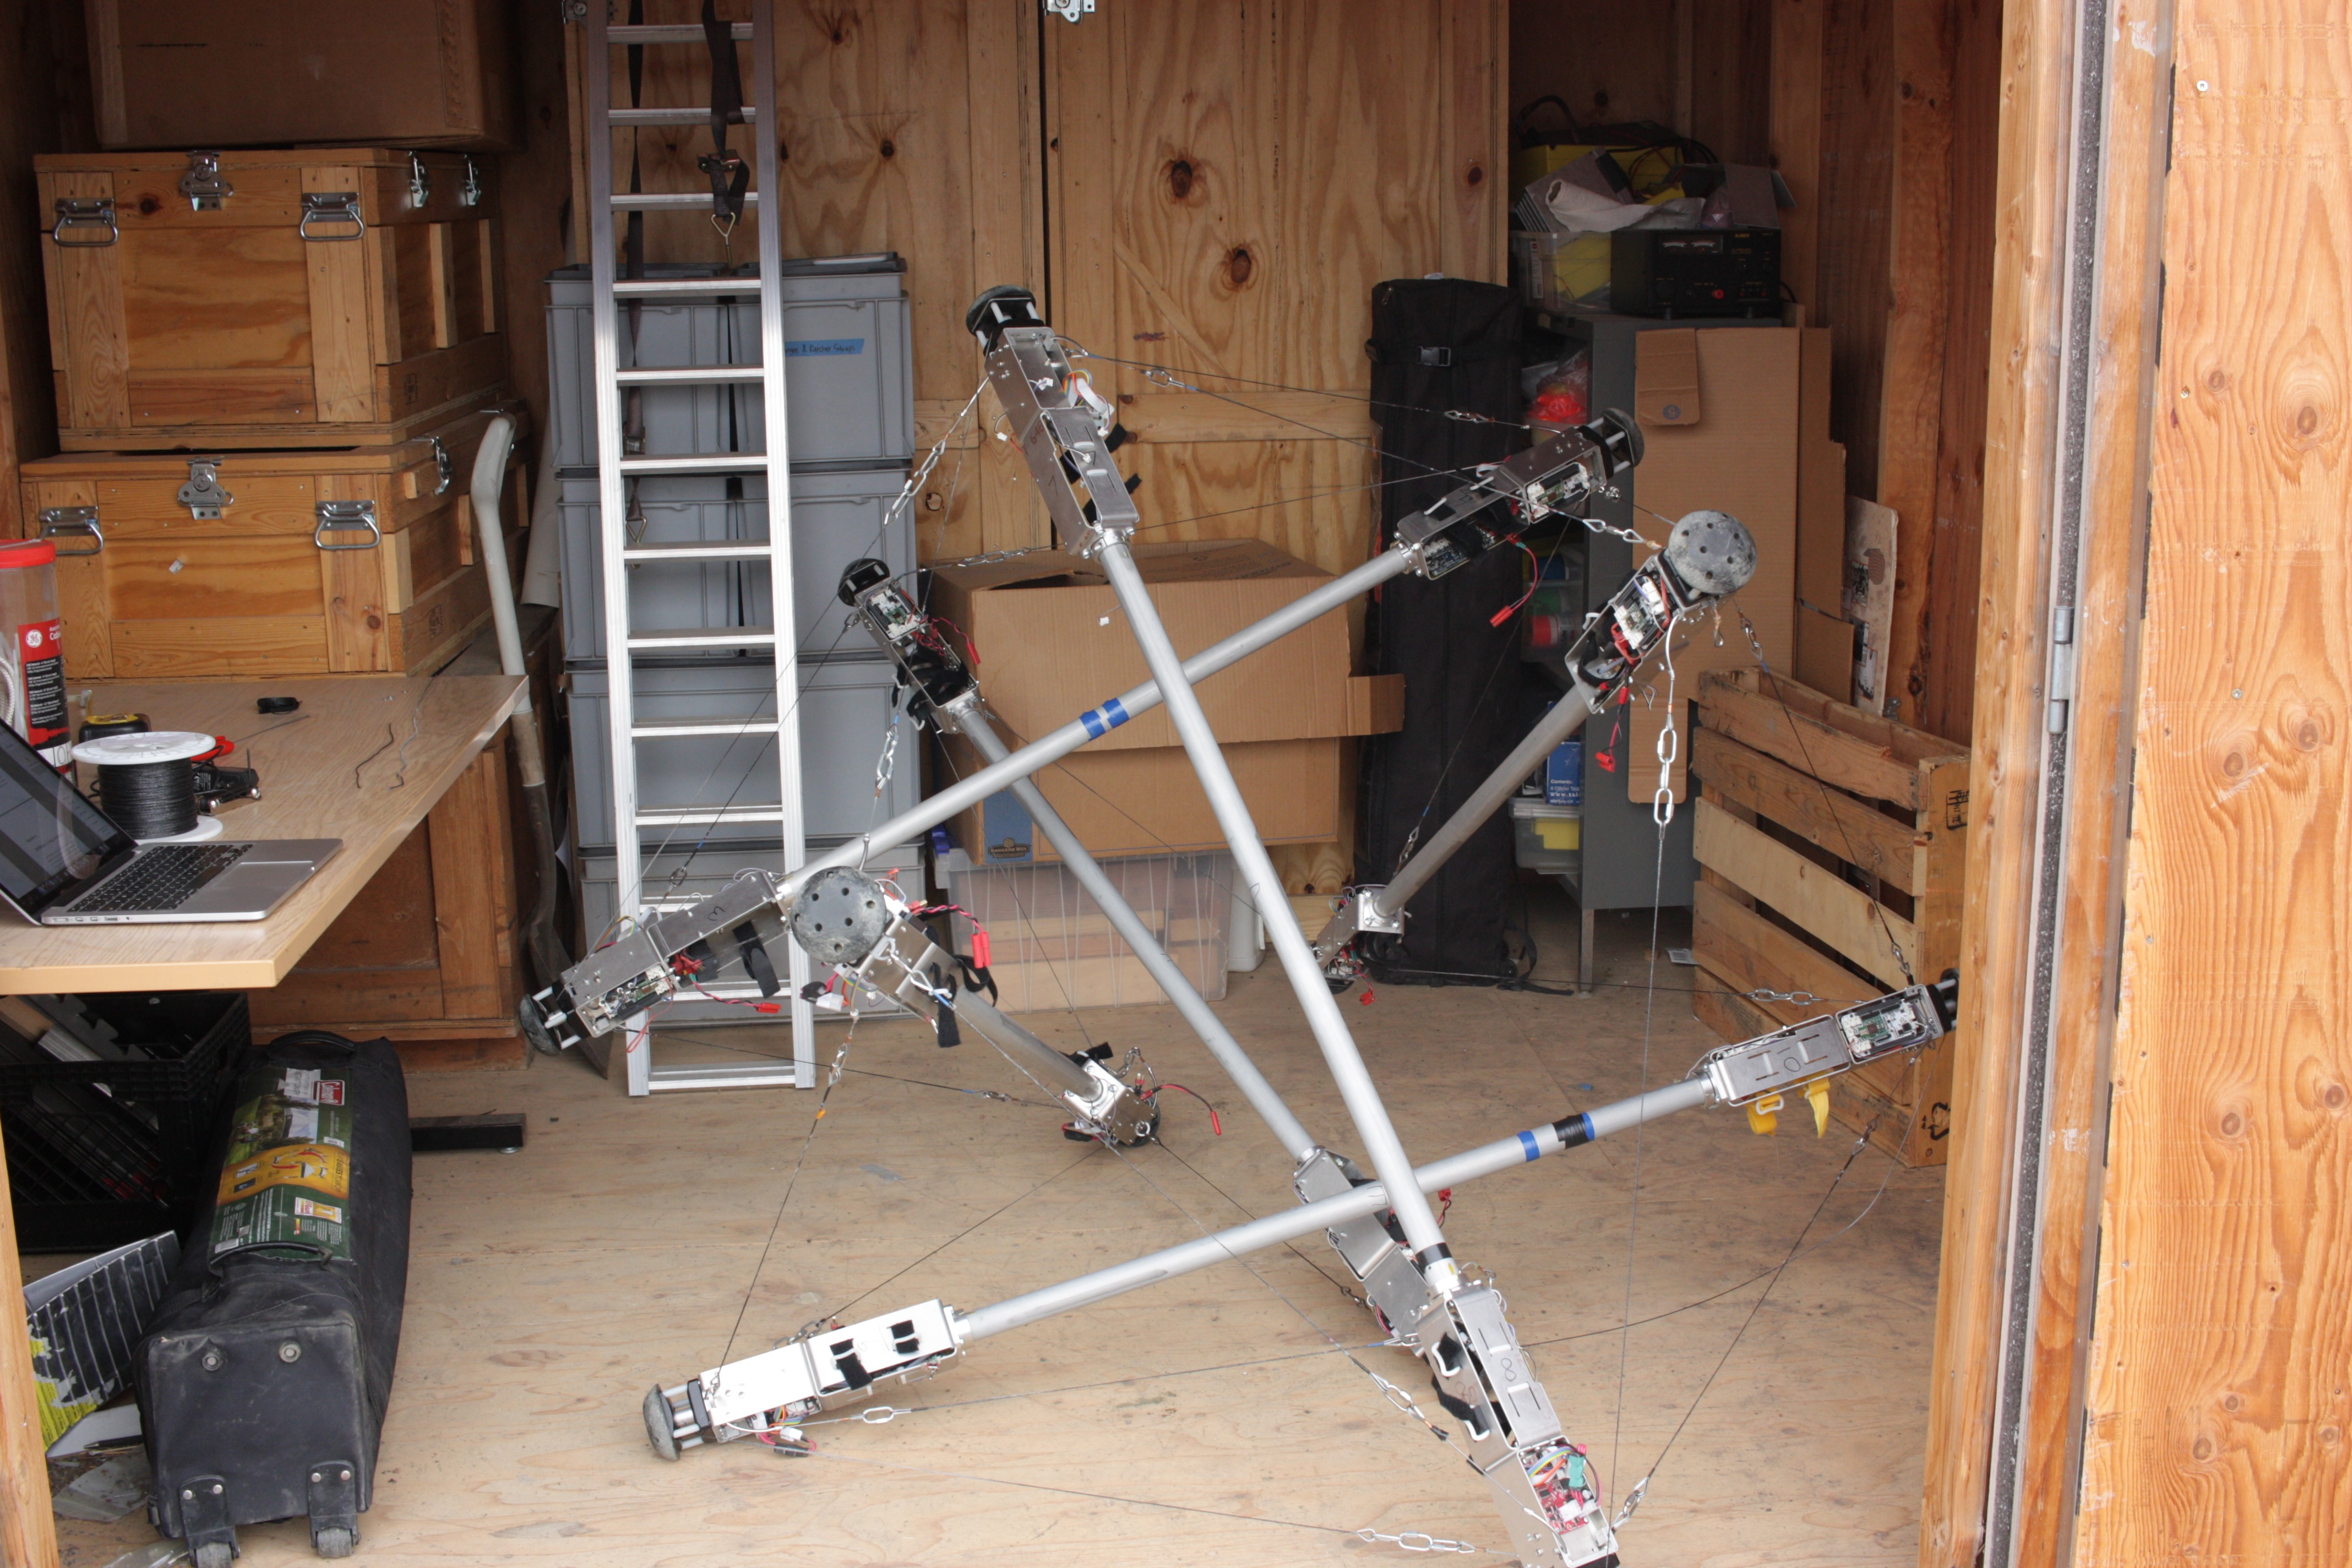
\includegraphics[width=0.9\linewidth]{tex/img/full_sb_down}%
\label{fig:sb_down}%
\caption{}
\end{subfigure}%

\caption{These figures show the hystresis effect due to friction on the \SB{}. \SB{} in the (a) figures has been lifted off the ground and gently placed back down so that all the springs in the system are allowed to reach equilibrium due to gravity. No extra force has been placed on the robot other than gravity. \SB{} in the (b) figures was arbitrarily pushed downwards on two of the top endcaps with enough force to deform the robot. It can easily been seen the that the internal friction does not allow for the robot to return to it's original state.}
\label{fig:cable_friction}
\end{figure}

Another limitation imposed by the cable routing system was the lack of design effort that went into the cable exit system.
Originally, it was designed to be a section of the nylon bowden cable housing sticking out of the robot to isolate the steel cable as it exited the MTR aluminum housing.
However, the angle in which the cable exits the system was never considered in the original \SB{} design. 
This failure meant that an exit angle of 90 degrees perpendicular to the rod as used for the cable exit.
Comparing this to the actual cable exit angle of approximately 30 degrees from perpendicular during normal operation meant that more than \(60\%\) of the tension force is imparted into the nylon cable and the aluminum housing exit hole.
When the cable would slide in and out of the exit point, the nylon tube quickly would sheer apart.
This then caused the steel cable to rub on the aluminum housing, which then would slowly saw into the housing.
Since there was not budget to redesign the whole routing system, a drop in replacement fix was required. 
The solution was to use a "break noodle" steel cable router typically used in bicycle braking systems.
This prevented the steel cable from cutting into to MTR housing, but it causes a bit more friction to get imparted into the whole cable system.
Figure~\ref{fig:cable_output} shows the cable exit point on \SB{} with the "break noodle" fix.

\begin{figure}[thpb]
      \centering
      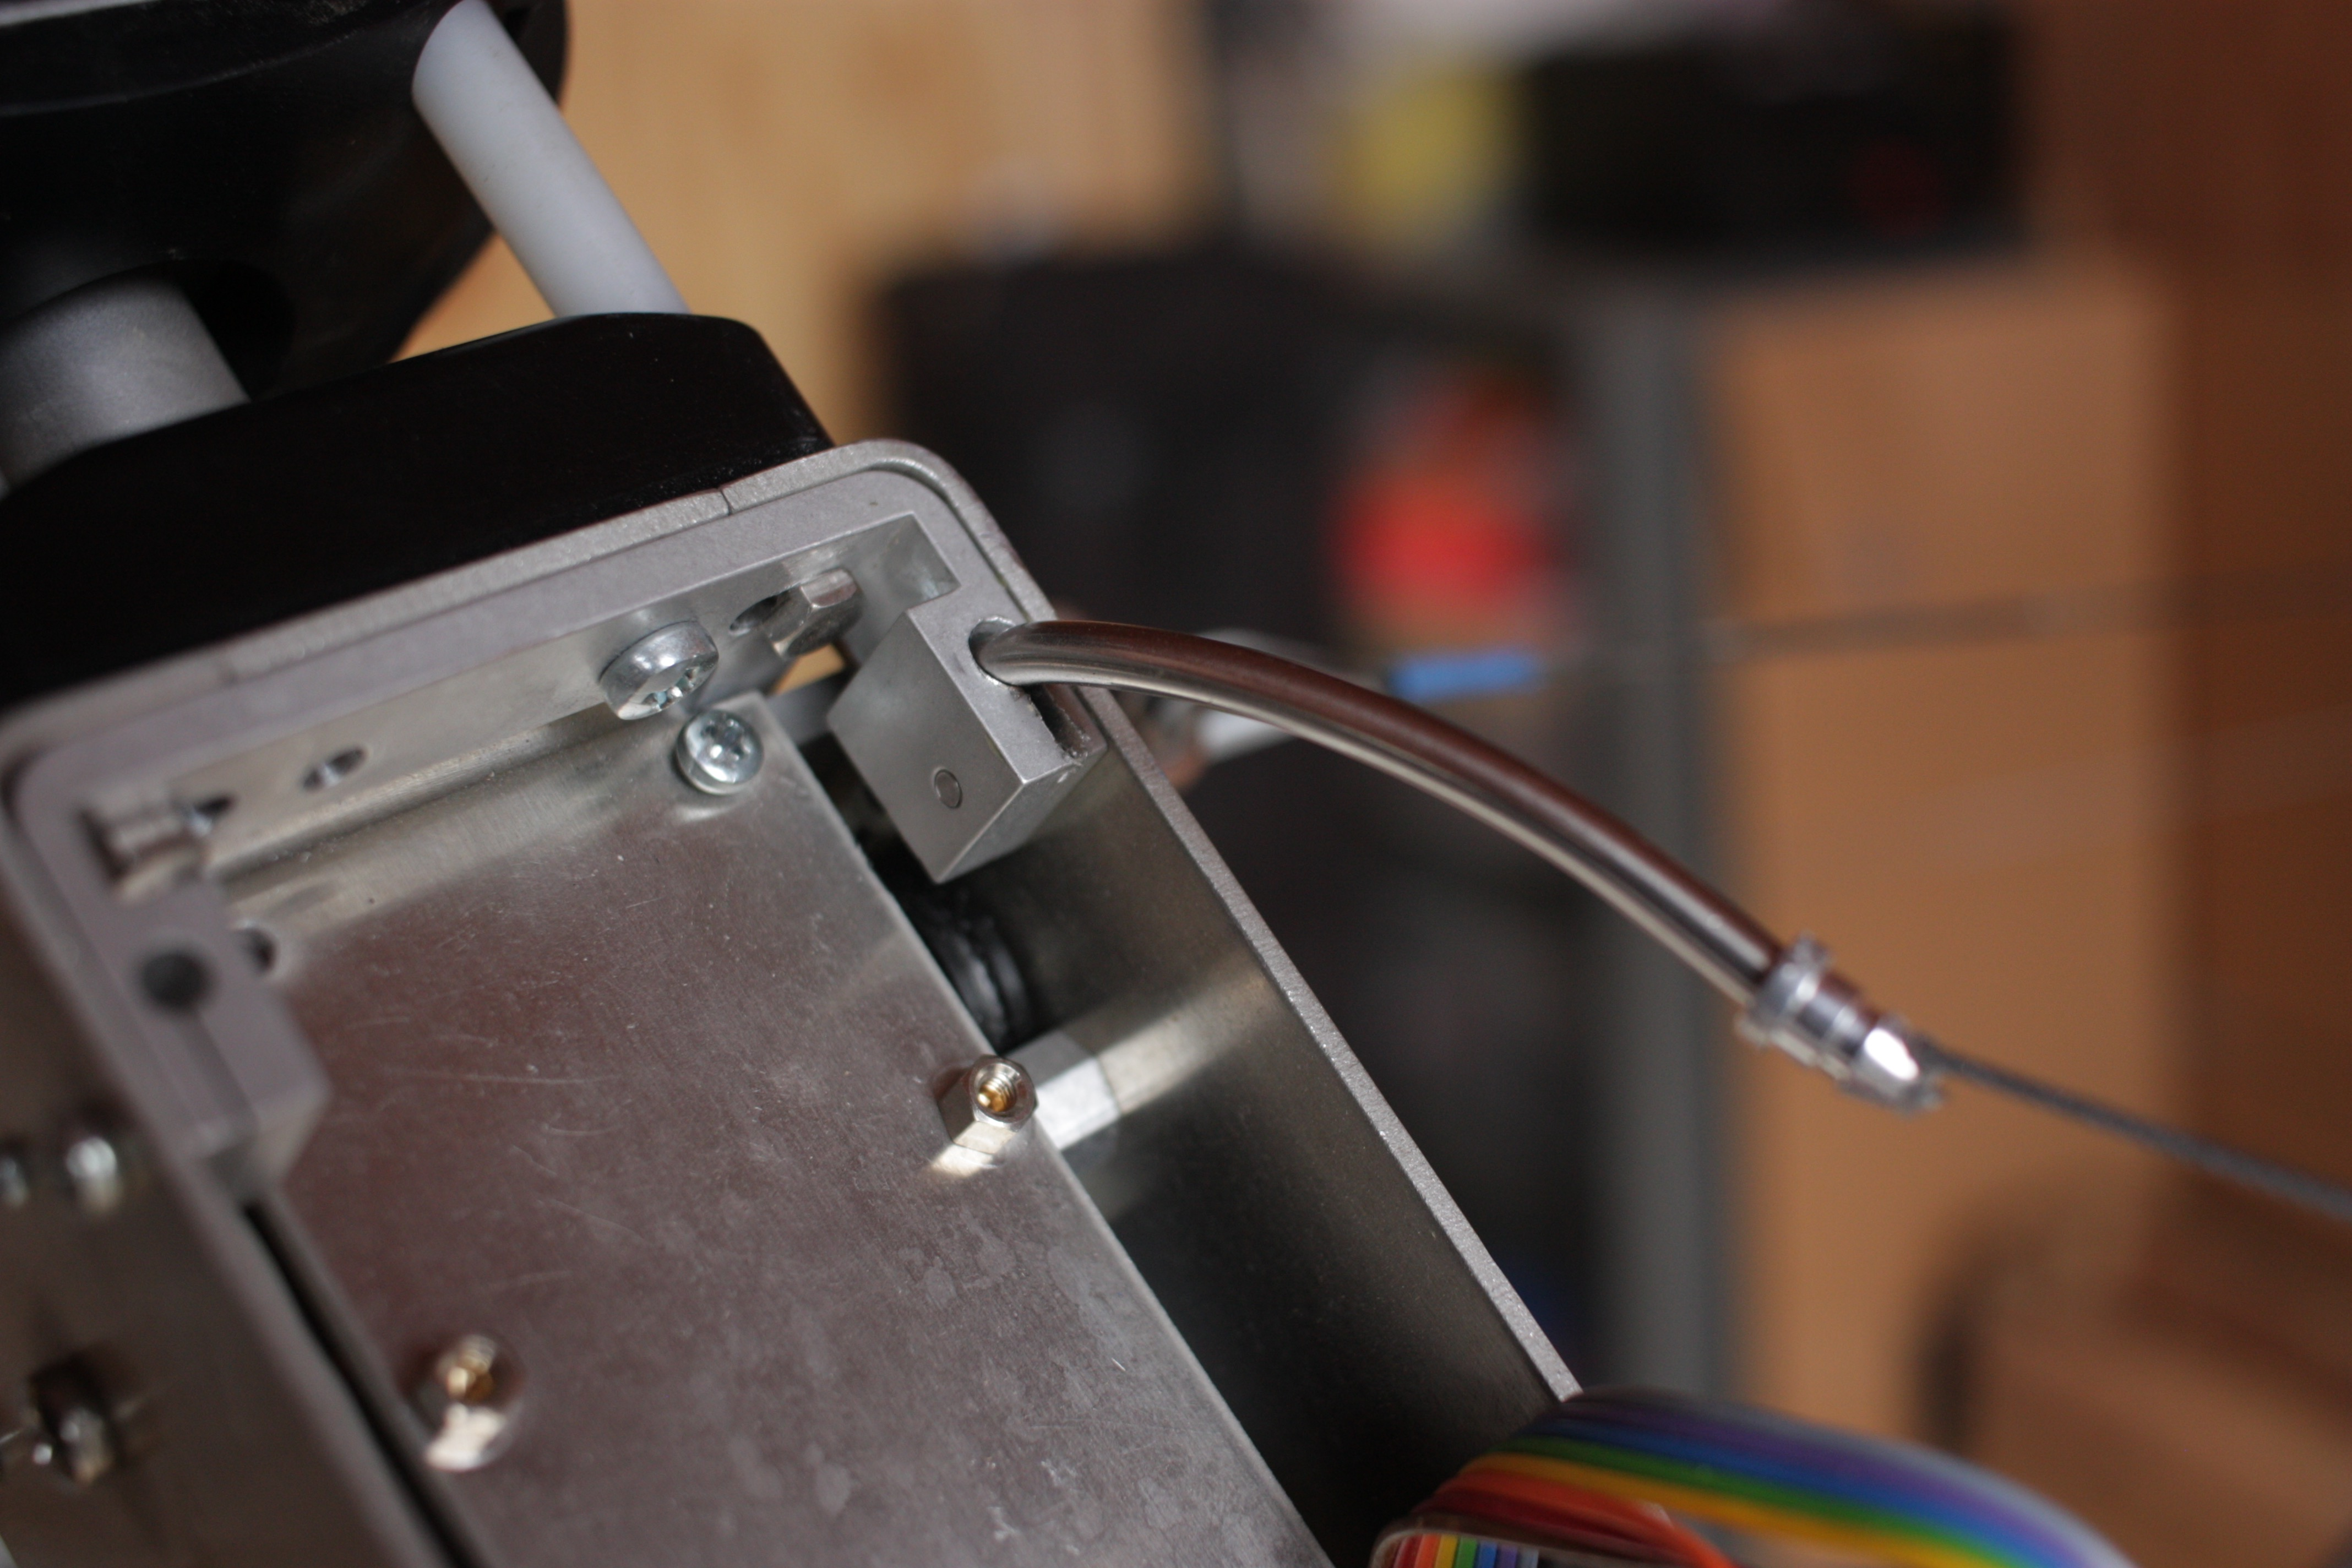
\includegraphics[width=0.8\columnwidth]{tex/img/bracket_cut}
      \caption{This figure shows the original exit point for the steel cable on \SB{} with the "break noodle" fix. The point of entry of the "break noodle" is can be seen where the aluminum of the bracket has been cut by the steel cable before the fix was applied.}
      \label{fig:cable_output}
\end{figure}

\subsection{Cable Tension}
\label{sec:cable_tension}
Another limitation on the system's performance is the larger than designed tensions seen on the individual cables.
This caused a limit on the maximum length each actuator imposes on a cable. 
Max cable tension on \SB{} was designed around a maximum continuous operating tension force of \(200N\) per cable.
The system was also designed to take intermittent forces \(50-75N\) higher than this maximum that would be caused by rolling.
These values were obtained through evaluating the tension forces derived from Iscen et al's control work within the NASA Tensegrity Robotics Toolkit~\cite{iscen2014flop}.
Atil used a simulated robot based on the initial design of \SB{}, which consisted of a total mass of \(18kg\) and each rod being \(1.5m\) in length. 
Comparing these values to those in table~\ref{design_req}, the final \SB{} parameters were different than the ones used to determine the operating tensions.
This was due to Atil's work was published quite early in the design process and not all the mechanical design aspects of the MTRs were finalized.
This discrepancy in weight caused the actual nominal operating tension to be around \(240N\) and the maximum operational tension to be above \(400N\).

The motors used in the final design of \SB{} were 100 watt Maxon motors as specified in table~\ref{motor_parameters}.
Each motor has a Maxon gearbox with a maximum continuous output torque of \(3Nm\) originally designed to be coupled to a spool with a diameter of \(30mm\).
Using the spool's radius and the robot's operating tensions listed above, the reaction torques applied to the gearboxes are calculated in equations~\ref{tau_nom} and~\ref{tau_max}.

\begin{align}
\tau_{nominal, 30mm} = 240N \times 0.015m = 3.6Nm \label{tau_nom} \\
\tau_{maximum, 30mm} = 400N \times 0.015m = 6.0Nm \label{tau_max}
\end{align}

These values are well above the continuous and peak torques that the motor's gearbox is rated to handle.
To keep from breaking all the motors when operating the robot, smaller diameter spools were designed. 
The trade off is that the cable actuation velocity is decreased, forcing the robot to move slower.
Decreasing the cable actuation velocity too far will result in a robot which will be incapable of achieving a continuous average forward velocity.
At the time, the only controller which moved a simulated \SB{} like robot with a continuous velocity was Iscen's work, which required a cable actuation velocity of \(30 cm/s\)~\cite{iscen2014flop}.
Thus reducing the speed below \(50\%\) could potentially be too slow to achieve continuous forward velocity.
The new spindles were then reduced to a spool diameter of \(18mm\) and the new torques are shown in equations~\ref{new_nom} and~\ref{new_max}.

\begin{align}
\tau_{nominal, 18mm} = 240N \times 0.009m = 2.7Nm \label{new_nom} \\
\tau_{maximum, 18mm} = 400N \times 0.009m = 3.6Nm \label{new_max}
\end{align}

This design still is not ideal, but is a compromise between reducing the reaction torque on the gearboxes and not reducing the actuation velocity too low.
The torques induced onto the gearbox could still go over the rated value during maximum tension scenarios, but reduces the actuation speed to \(47\%\) of the original value set by Iscen.
To further reduce the reaction torques applied to the gearboxes, a maximum position of cable change was set to keep the reaction torque applied my any one motor to be within the nominal spool reaction torque in equation~\ref{new_nom}.
Though experimentation, the limit was found to be \(40cm\) of cable change from a pretension value in each cable of \(100N\).

\subsection{Cable Material}
The choice of external cable material used on \SB{} made some complications in the long term use of the system.
The material used is a \(1.3mm\) diameter braided hollow core Vectran cable.
This cable has excellent material properties for a system which requires light and strong cables with near zero creep.
However, the cable has a high coefficient friction and will undergo tensile fractures when exposed to large amounts of stress.
This causes the many thin fibers to fray, eventually leading to loss in overall tensile strength and eventual failure. 
In \SB{}, this usually occurs at the cabling closest to the spool. 
Since this small length of cable always experiences high stress due to wrapping around the spool, the cables fray quite rapidly and break.
The frequency of this happening depends on how many times that particular cable is used.
On average it has become an expectation that a single cable will break after at least three hours of actuation on that single cable. 
Figure~\ref{fig:cable_break} shows different stages of the vectran cable as it wears to breakage.

\begin{figure}[thpb]
      \centering
      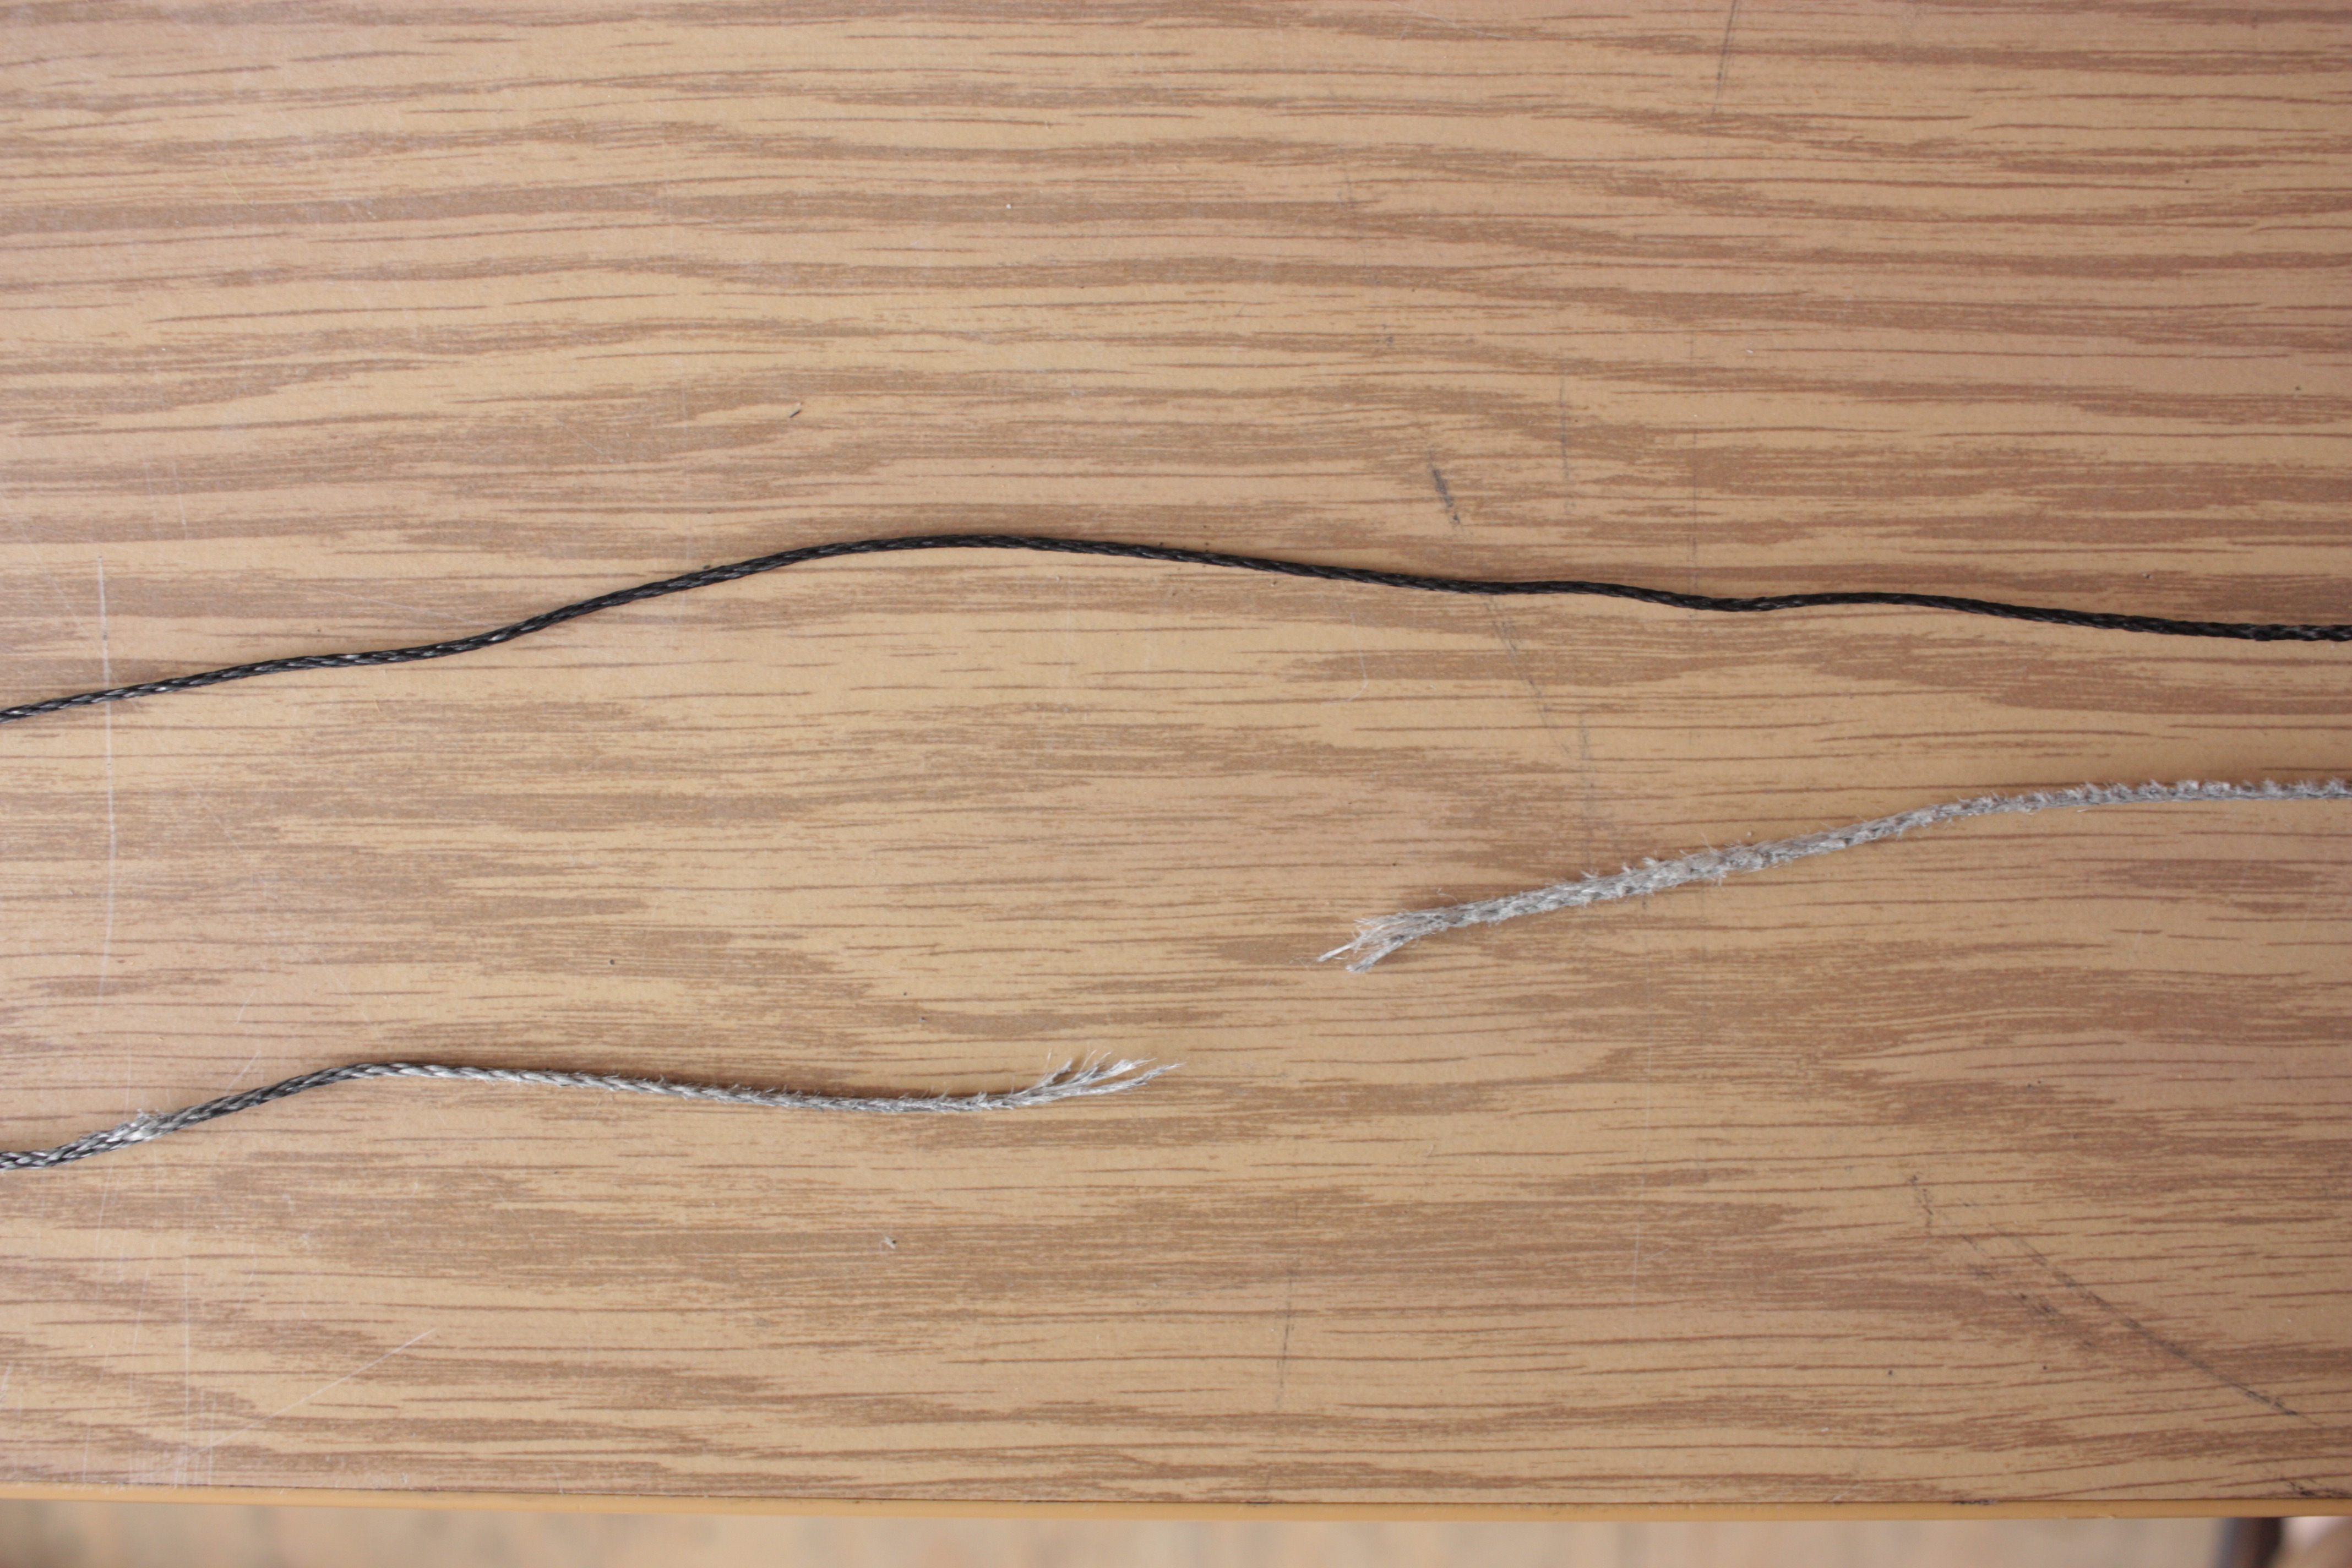
\includegraphics[width=0.8\columnwidth]{tex/img/broken_cable}
      \caption{This figure shows how wear on the cable. The vectran cable's protective outer coating wears off during use which then allows for the individual fibers to break weakening the entire cable. Eventually this wear will degrade the max holding tension to the point of failure. The black cable is a new vectran cable and the cable below shows the black coating worn away and a breakage point. The bottom cable is from an actual failure on the system during a run. Since the system can absorb forces, when the cable breaks the stored energy gets distributed into the robot and no violent backlash is experienced.}
      \label{fig:cable_break}
\end{figure}

\subsection{Force Sensors}
\label{force_sensing_failure}
\SB{} was designed to have three force sensors per MTR system to sense forces being applied by the motor, the distal actuated cable, and the distal passive cable.
Since the system had a constrained budget, purchasing off the shelf force sensors was out of the budget and custom sensors were implemented.
Figure~\ref{fig:force_sensors} shows the designs for each force sensor.

\begin{figure}[thpb]
      \centering
      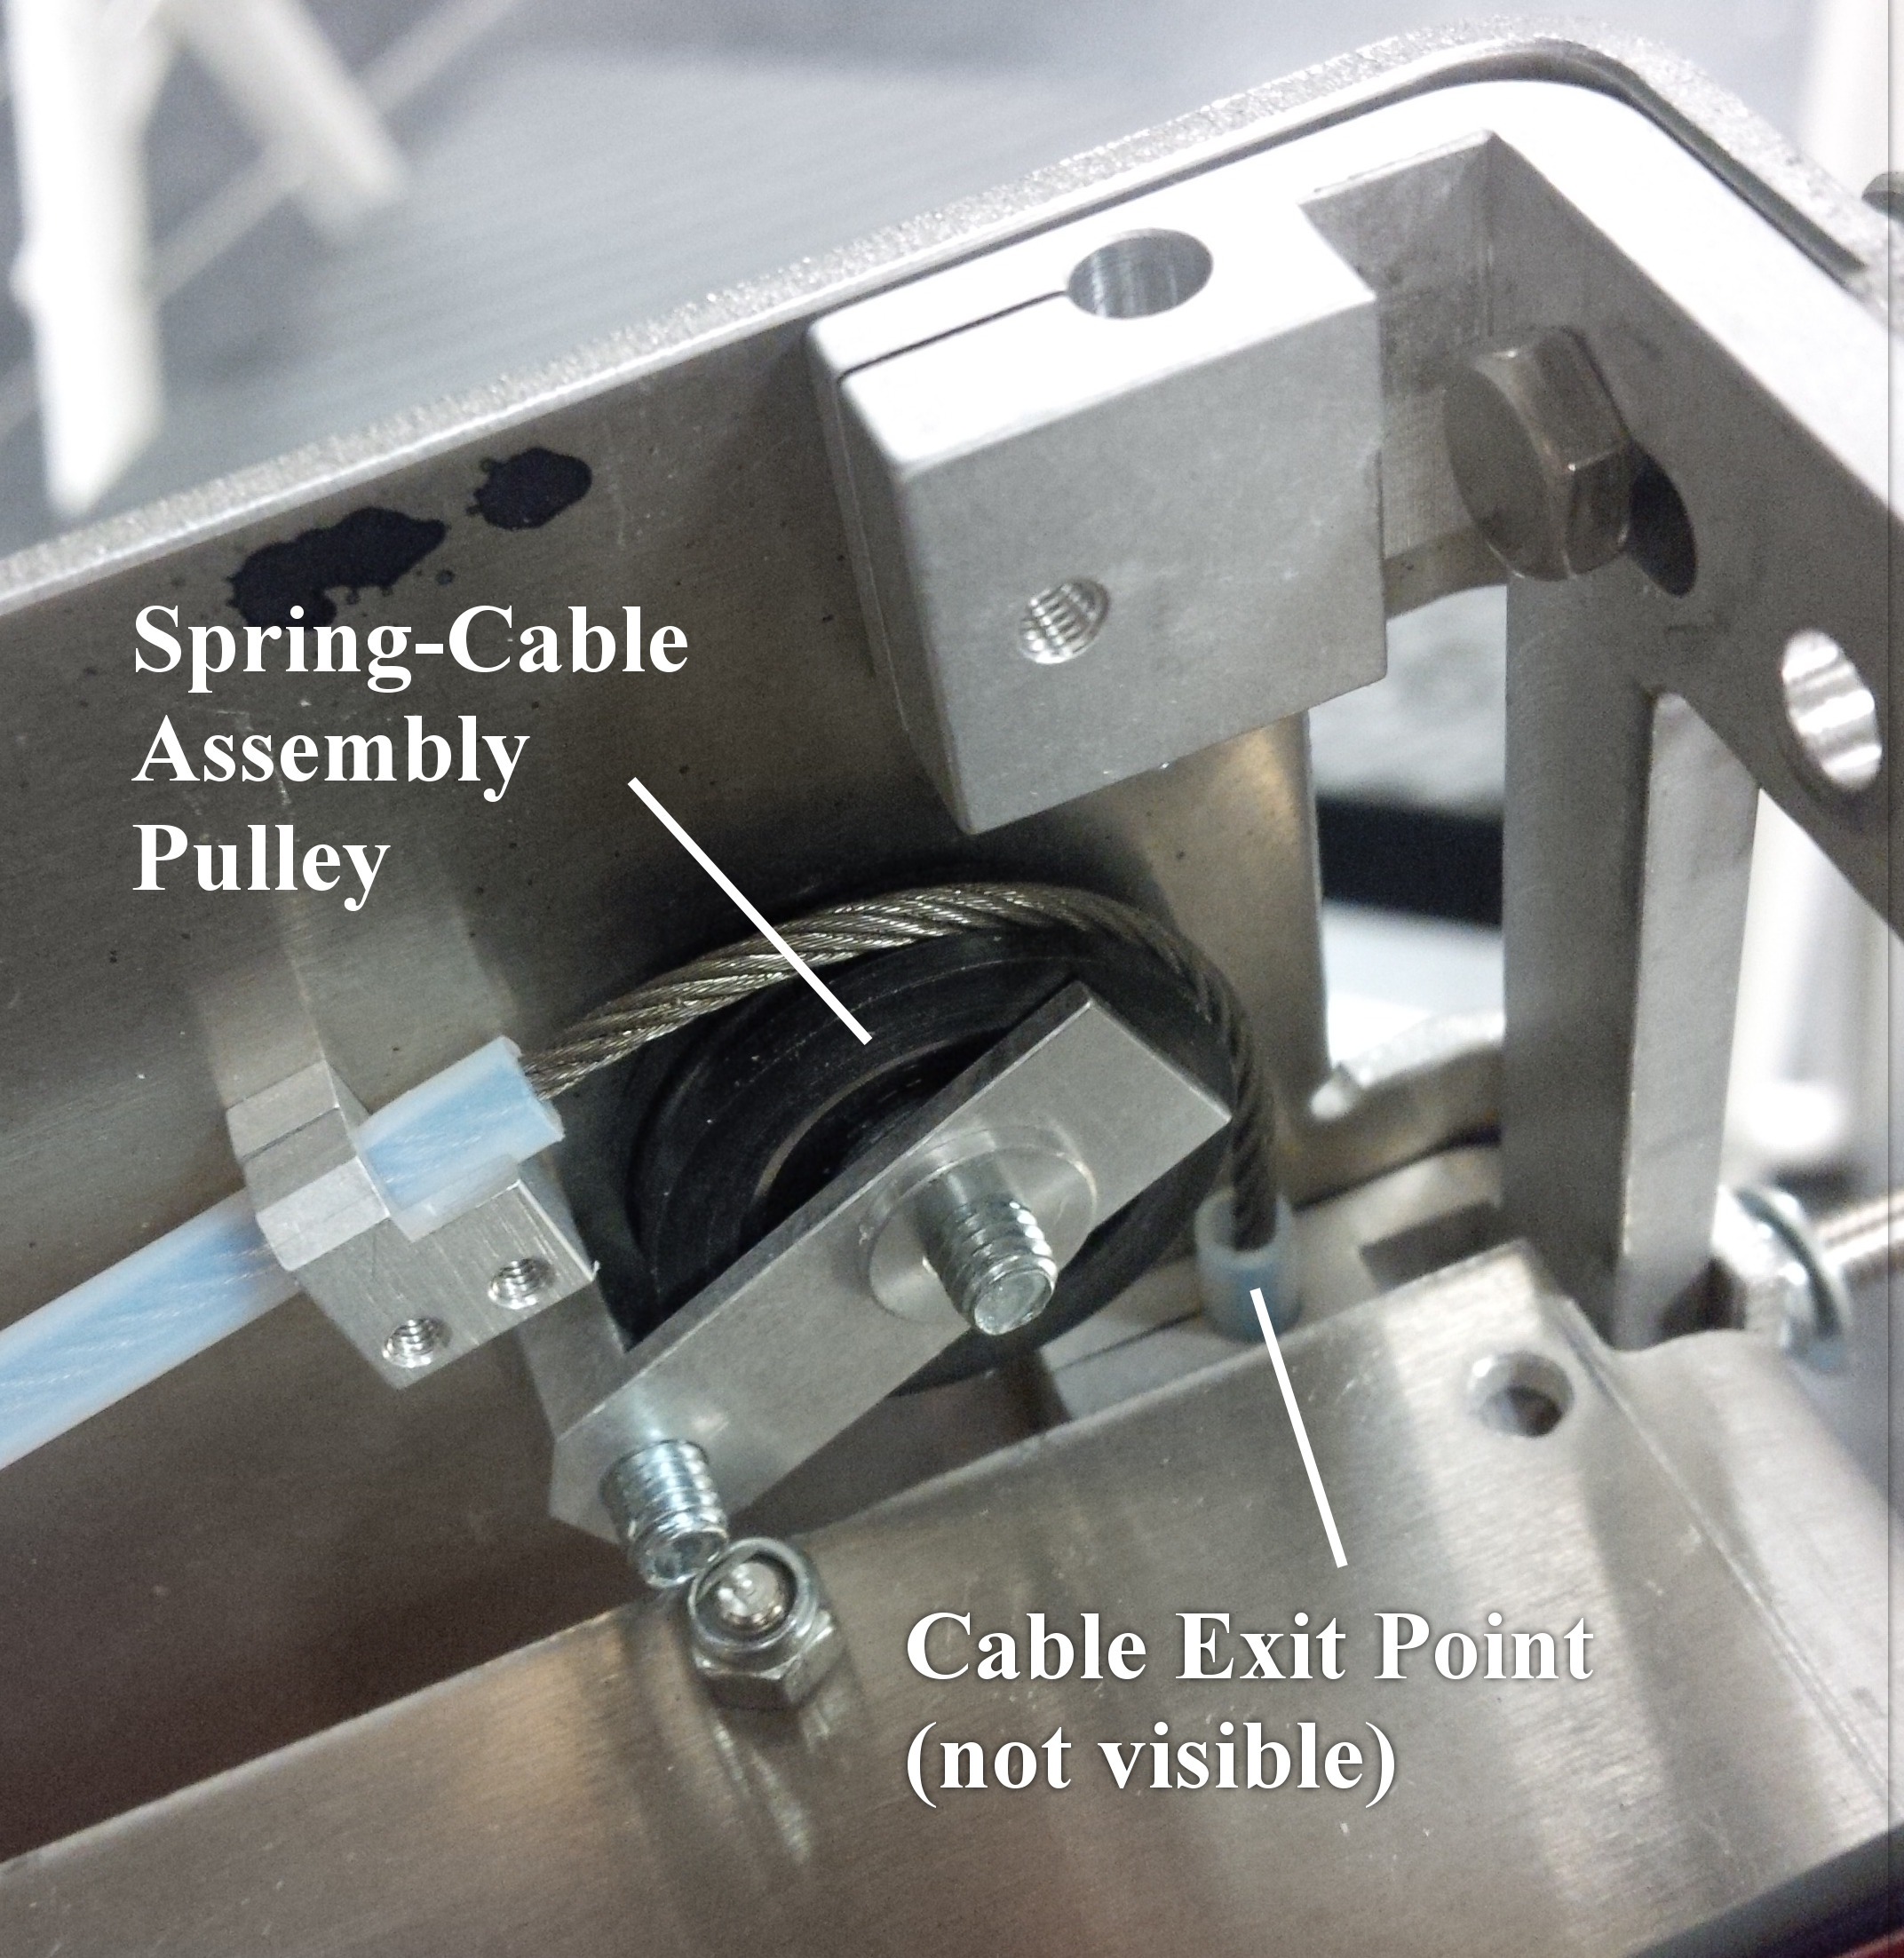
\includegraphics[width=0.6\columnwidth]{tex/img/cable_pulley_bearing_labelled_fixedfonts}
      \caption{\textcolor{red}{Temp. figure. Show each force sensor.}}
      \label{fig:force_sensors}
\end{figure}

\paragraph{Dynamic Torque Sensor Testing}
\begin{figure}[thpb]
      \centering
      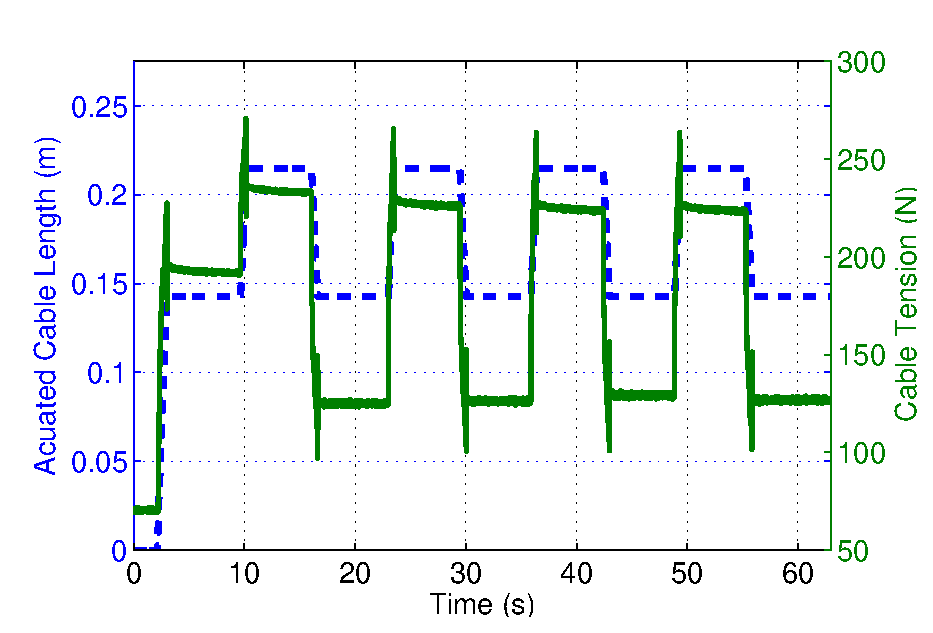
\includegraphics[width=0.8\columnwidth]{tex/img/ICRA2015_dynamic_sensor_test}
      \caption{Motor mount torque sensor data and motor position data recorded during a square wave input position trajectory for a single motor. This plot shows measured tension from the sensor and cable length from motor encoder measurements as a function of time for this dynamic movement.}
      \label{fig:sensor1data}
\end{figure}

This test was performed to demonstrate the force sensors' ability to capture data under dynamic motion.
Figure~\ref{fig:sensor1data} shows a plot of sensor data from one end cap whose motor is commanded in a square-wave position trajectory.
The position trajectory had a period of \SI{13}{\second}, and oscillated between \SI{10}{\radian} and \SI{15}{\radian} of the output shaft measured before the gearbox, by the encoder.
The trajectory of sensor torque values reasonably tracks the position square wave: the commanded position trajectory starts at 10 seconds and ends at 62 seconds, as does the sensed tension square wave.
The overshoot on the torque sensor measurements is due to the system inertia and spring dynamics.

\paragraph{Global Force Redistribution Sensor Testing}
\begin{figure}[thpb]
      %\vspace{-0.5cm}
      \centering
      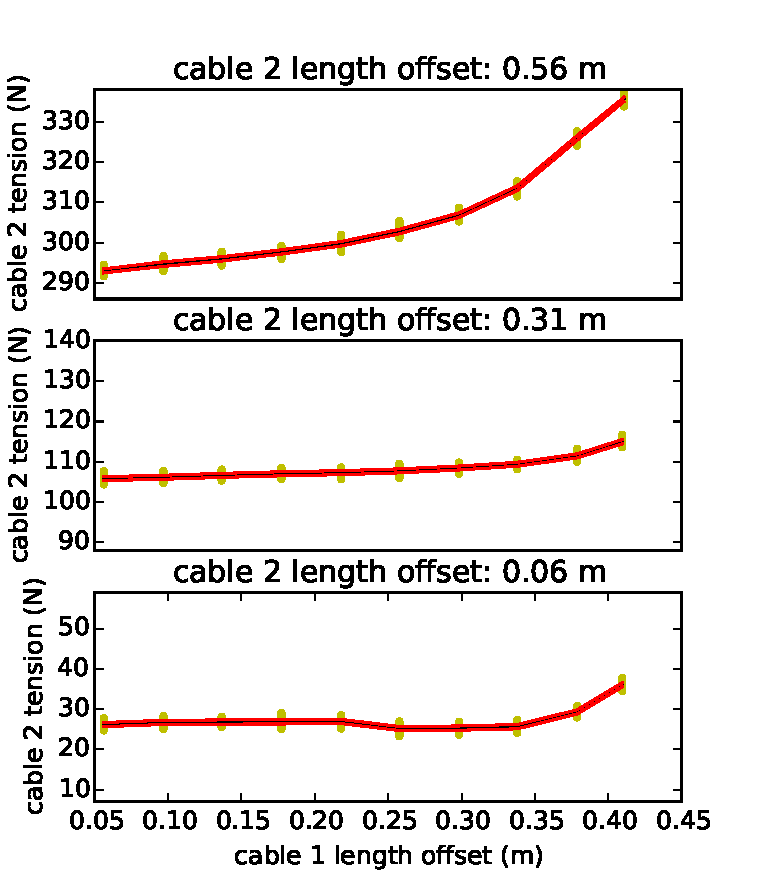
\includegraphics[width=0.55\columnwidth]{tex/img/sensor2_original}
      \caption{Global force redistribution test. Yellow marks are the means of roughly 5,000 tension sensor measurements of \emph{cable 2} opposite that which is actuated (\emph{cable 1}.) The black line shows the linear interpolation between points, with the red boundary as standard deviation. The pretension in the sensed cable is adjusted in each test, showing measurement sequences at increasing pretensions.}
      \label{fig:sensor2data_forcedistribution}
\end{figure}

A test was performed to validate the distribution of tension throughout the system, and to show that all sensors can work in conjunction simultaneously.
Figure~\ref{fig:sensor2data_forcedistribution} shows tension readings from a different motor-mount torque sensor on the opposite side of \SB{} (Cable 2) from a cable which is being retracted (Cable 1.)
Cable 2 was not actively actuated during each test.
For each plot in Figure~\ref{fig:sensor2data_forcedistribution}, the actuated cable was retracted with various step inputs marked in the figure.
Each data point in this figure (yellow) was collected by averaging data from the sensor board for a total of 5 seconds at 1 kHz, after waiting 2 seconds after the step input actuation to avoid dynamic effects.
These tests were done with different levels of pretension on the sensed cable: this pretension was adjusted by changing the length of the sensed cable.
Though the lower-pretension tests show smaller changes in readings, the higher pretensions show increasing readings which demonstrate the ability to sense forces throughout the tension network in pseudo-equilibrium states, as well as \SB{}'s passive force redistribution properties.

\paragraph{Force Sensing Viability}
The force reaction sensor was the only custom sensor to accurately sense the forces applied.
However, inconsistencies in manufacturing this sensor made calibration of each sensor extremely difficult.
This coupled with not being robust to handling, it was extremely difficult to get all twelve sensors working at one time.
A single sensor could be made, calibrated and functional for about a day or two after which the sensor's strain gages would shift.
This either would making the calibration no longer valid or be such an shift, that the sensor would no longer be functional.
Due to these set backs, the force sensors were disregarded as viable sensors to be used on the system.

\section{Electrical Evaluation}
% \textcolor{red}{
%  - Motor Board design
%    > lacked fully functionality
%    > large board with large connectors
%    > not quite fast enough for FoC
%  - Sensor Board desgin
%    > Wifi module never worked, became hack for DWM module - not enough clearance for antenna
%    > ADC never used because of Torque and Force sensors not working
%  - Power Board design
%    > Large design and no connectors for main power inputs
%    > Too many 5.5V outputs
%    > nRF24 chip mounting is problematic 
% }

For the most part, all the electronic boards on \SB{} functioned as designed with only the motor control board (motor board) having lasting issues that hindered the performance of the system.
The motor board was suppose to be a low cost solution to achieve position, velocity, and torque control utilizing the Field Oriented Control (FOC) method to commutate our brushless DC motors.
A third party start-up company was tasked with the design of the motor board.
It took the company many attempts to get a working version for just position control, with the initial delivery causing motors to generate excessive heat due to shorting the windings during commutation.
After a quick redesign and manufacturing new boards, position control was achieve with pretty good results.
However, the company went out of business after delivering working motor control boards and never completed their implementation of the other control methods.
Because of the issues stated in section~\ref{force_sensing_failure}, torque control could not have been implemented.

% The main feature of the sensor board was to monitor and control any of the sensors required on \SB{} by a dedicated processor.
% This was to insure that none of the critical safety features would be hindered by sensor tasks.
% Most of the board's functions work as expected.
% %However the analog to digital converter became useless after all the force sensors failed as explained in section~\ref{force_sensing_failure}.
% The only real issue when using this board steams from the re-purposing of the XBee WiFi headers for controlling a DecaWave DWM1000 module.
% This placed the module's antenna too close to the robot to effectively get ranging data in all directions.
% A better design would have place the antenna such that one complete side of the sensor was not completely blocked by the MTR module. 


% \subsection{Motor Board}
% The motor control board for \SB{} never worked as designed and eventually limited the capabilities of the system.

\section{Communications Evaluation}
% \textcolor{red}{
%  - CAN Bus 
%    > too slow for fast control and lots of data
%    > large overhead for processors utilizing driver code (CANOpen)
%  - BBB
%    > slow to boot
%    > draws lots of power
%    > Wifi dongle has connection issues
%    > big and heavy for what the board does
% }

\end{appendices}